\documentclass[oneside,final,14pt,a4paper]{extreport}

\usepackage{multirow}
\usepackage[utf8]{inputenc}
\usepackage[russianb]{babel} % адаптация русского языка
\usepackage{vmargin} % настройка размера полосы набора
\setpapersize{A4}
\setmarginsrb{2cm}{2cm}{2cm}{2cm}{0pt}{0mm}{0pt}{13mm} % {левое поле}{верхнее поле}{правое поле}{нижнее поле}{колонтитулы}{колонтитулы}{колонтитулы}{номер страницы}
\usepackage{indentfirst} % отделять первую строку раздела абзацным отступом
\usepackage{graphicx} % подключение библиотеки для работы с внешними картинками
\usepackage{setspace} % для изменения межстрочного интервала
\sloppy % выравнивание текста
\setstretch{1.5} % устанавливаем межстрочный интервал

\usepackage[labelsep=space]{caption}
\addto\captionsrussian{\renewcommand{\figurename}{\CYRR\cyri\cyrs\cyru\cyrn\cyro\cyrk}} % меняем "Рис." на "Рисунок"

%\renewcommand{\thetable}{\thechapter.\arabic{table} ---} % добавить дефис после номера таблицы


\usepackage {titlesec}
\titleformat{\chapter}{\hyphenpenalty=10000\normalfont\huge\bfseries\flushleft}{\thechapter\space\space}{0pt}{\huge} % меняем заголовок для команды \chapter и запрещаем переносы слов

\usepackage{floatrow}
\floatsetup[table]{capposition=top} % разместить подпись к таблице наверху
  
\makeatletter
\renewcommand{\@biblabel}[1]{#1\space} % Заменяем библиографию с [number] на просто number:
\makeatother

\newcommand{\Expect}{\mathsf{E}}
\newcommand{\MExpect}{\mathsf{M}}

\AtBeginDocument{\renewcommand\tablename{Таблица}} % переименовать Таб. на Таблица







% ---------------------------------------------------------------------------------------------------------------
% ---------------------------------------------------------------------------------------------------------------
% ---------------------------------------------------------------------------------------------------------------
% Начало документа
\begin{document}





% ТИТУЛЬНЫЙ ЛИСТ НАЧИНАЕТСЯ
\thispagestyle{empty}
\begin{titlepage}

\begin{figure}
	\centering
	
\includegraphics[width=0.5\textwidth]{msu}\\
\end{figure}

\begin{spacing}{1.0} % устанавливаем межстрочный интервал
\begin{center} % центрируем текст
	{\small
		Московский государственный университет имени М.В. Ломоносова \\
		Факультет вычислительной математики и кибернетики \\
		Кафедра автоматизации систем вычислительных комплексов \\
	}
	\vspace{4cm}
	{\large Романов Андрей Романович \\}
	\vspace{1cm}
	{\large\bfseries
	    Разработка системы валидации виртуальных сетевых сервисов \\
	}
	\vspace{1cm}
	МАГИСТЕРСКАЯ ДИССЕРТАЦИЯ
\end{center}
\vfill
\begin{flushright}
\begin{small}
	{\bfseries Научный руководитель: \\}
	к.ф.-м.н. \\
	В.А. Антоненко \\
\end{small}
\end{flushright}

\vfill

\centerline{Москва, 2018}
\end{spacing}
\end{titlepage}
% ТИТУЛЬНЫЙ ЛИСТ ЗАКАНЧИВАЕТСЯ

\setcounter{page}{2}  % начать нумерацию страниц с 2





\chapter*{Аннотация}
В данной работе рассматривается проблема валидации виртуальных сетевых сервисов.

В рамках данной работы был проведен обзор существующих решений в части валидации виртуальных сетевых сервисов, а также обзор языков спецификаций виртуальных сетевых функций. Разработана архитектура приложения, позволяющего выполнять анализ виртуальных сетевых функций и выдавать подходящую с точки зрения удовлетворения пользовательских требований конфигурацию виртуальных сетевых сервисов. Проведено экспериментальное исследование влияния разработанного модуля валидации на время получения стабильной подписки на виртуальный сетевой сервис.





% Оглавление
\def\contentsname{Содержание} % переименовать Оглавление в содержание
\tableofcontents % генерация оглавления





\chapter*{Введение}
\addcontentsline{toc}{chapter}{Введение} % добавление Введение в оглавление
В современных сетях функционирует достаточно большое число сетевых функций: маршрутизация (routing), трансляция сетевых адресов (NAT), сетевой экран (firewall), туннелирование (VPN), защита от DDoS атак (anti-DDoS), антиспам (antispam) и многие другие. Программную реализацию большинства из них невозможно отделить от аппаратной составляющей. Такое положение дел приводит к ряду проблем. 

В случае нехватки мощностей можно использовать сразу несколько устройств. Рекомендуется использовать устройства от одного производителя, а лучше одной и той же модели. В этом случае уменьшается риск несовместимости интерфейсов. Все это приводит к зависимости пользователей сетевого оборудования от производителя.

При возникновении необходимости в дополнительной функциональности требуется приобретать оборудование, часть функциональности которого будет избыточной. Например, пусть имеется маршрутизатор без поддержки протокола VXLAN и нет возможности вносить изменения в прошивку устройства. При этом туннелирование трафика необходимо осуществлять с помощью заданного протокола. Тогда необходимо приобретать новое оборудование, однако новый маршрутизатор будет обладать теми же стандартными сетевыми функциями такими как NAT, routing, DNS, DHCP, что и старый маршрутизатор. Таким образом, новое устройство содержит в себе избыточную функциональность.

Поддержку программной части сетевого оборудования осуществляет команда разработчиков компании-производителя, и пользователь в большинстве случаев не может самостоятельно вносить изменения из-за закрытости программного обеспечения оборудования. После окончания срока поддержки сетевого устройства пользователь полностью теряет возможность изменять программную составляющую оборудования. Поэтому остается единственной выход --- приобретение нового устройства.

Для увеличения мощностей одной сетевой функции требуется увеличивать число физических устройств. Что снова ведет к проблеме избыточной функциональности новых устройств. При этом при обычных (не пиковых) нагрузках часть устройств простаивает. Здесь проявляется невозможность динамического масштабирования сетевых функций в зависимости от нагрузки.

Таким образом, можно выделить ключевые проблемы организации работы сетевых функций:
\begin{itemize}
	\item использование оборудования с избыточной функциональностью;
	\item расчет производительности инфраструктуры исходя из максимально возможной нагрузки;
	\item простаивание оборудования в случае, если нагрузка не является пиковой;
	\item зависимость от производителя оборудования:
	\begin{itemize}
	    \item техническое обслуживание;
	    \item устаревание ведет к необходимости замены оборудования;
	    \item невозможность модифицировать функцию без вмешательства производителя.
	\end{itemize}
\end{itemize}

Для решения указанных выше проблем была разработана концепция виртуальных сетевых функций, речь о которой пойдет в следующем разделе. 




\chapter{Концепция виртуальных сетевых функций}
\label{chap:nfv}
Концепция виртуальных сетевых функций (Network Function Virtualization, NFV\cite{bib:nfv:white-paper}) позволила бы решить указанные выше проблемы, автоматизировав размещение инфраструктуры и развертывание программного обеспечения в облаке. NFV -- это концепция сетевой архитектуры, предлагающая виртуализировать классы сетевых функций в виде составных элементов, которые могут быть связаны в цепочку для создания телекоммуникационных услуг (сервисов). Концепция виртуализации сетевых функций была предложена в 2012 году Европейским институтом телекоммуникационных стандартов\cite{bib:nfv:white-paper}.

Под виртуализацией сетевых функций понимается разделение программной и аппаратной составляющих сетевых функций. При этом аппаратная составляющая заменяется на виртуальную инфраструктуру (которая включает в себя: виртуальные машины, контейнеры, виртуальные хранилища и виртуальные сетевые элементы), а программная составляющая (программное обеспечение функции) запускается на этой виртуальной инфраструктуре. Такие сетевые функции называются виртуальными сетевыми функциями (Virtual Network Function, VNF). В качестве примера можно привести такую виртуальную сетевую функцию как система предотвращения вторжений Snort\cite{bib:snort}. Она может состоять, например, из одной виртуальной машины с программой Snort.

Программа, которая поддерживает концепцию NFV, занимается управлением виртуальными сетевыми функциями, позволяет создавать, размещать, изменять, удалять цепочки виртуальных сетевых функций, называется NFV платформой. Использование NFV платформы имеет смысл только при наличии интегрированных в нее виртуальных сетевых функций.

Необходимо учесть, что не все функции можно эффективно виртуализировать. Примитивные операции с сетевым трафиком, такие как перенаправление пакета с одного порта на другой и другие низкоуровневые действия с сетевыми пакетами, которые надо выполнять наиболее часто и быстро, условно выделяют в плоскость передачи (Data Plane). Наоборот, различные протоколы обнаружения соседства, маршрутизацию, механизмы балансировки, телеметрию, авторизацию, аккаунтинг относят к плоскости управления данными (Control Plane), так как здесь уже требуются различные алгоритмы работы с трафиком и не так критична скорость обработки сетевых пакетов. Таким образом, чем меньше совершается операций вида Data Plane и чем больше вида Control Plane, тем целесообразнее перенести рассматриваемую сетевую функцию в NFV платформу. И, наоборот, чем больше Data Plane и чем меньше Control Plane операций, тем лучше оставить сетевую функцию привязанной к оборудованию.

Интеграция существующей сетевой функцией может быть связана с необходимостью доработки ее программного обеспечения для работы в виртуальной среде. Здесь имеется ввиду использование стандартных, не привязанных к конкретной аппаратуре, интерфейсов драйверов и библиотек.


\section{Дескрипторы функций}
Концепция NFV предполагает динамическое изменения состава зарегистрированных в платформе виртуальных сетевых функций. Все функции в NFV платформе представляются дескрипторами --- контейнерами, в которых хранится вся необходимая информация, для управления жизненным циклом виртуальной сетевой функции. Дескриптор включает в себя:
\begin{itemize}
    \item спецификацию топологии виртуальной инфраструктуры;
    \item параметры размещения и схема настройки функции;
    \item доступные действия над функцией;
    \item алгоритмы управления подключением пользователей к функции;
    \item алгоритмы действий в случае перегрузки и/или недоступности функции.
\end{itemize}

Впоследствии функция может устареть и перестать использоваться, тогда ее удаляют из NFV платформы. В случае если пользователь желает использовать какую-либо функцию и при этом отправляет соответствующий запрос в NFV платформу, то говорят, что пользователь совершает подписку на виртуальную сетевую функцию. Указанная в дескрипторе функции информация позволяет NFV платформе:
\begin{itemize}
    \item по требованию осуществлять подписка пользователя на указанную функцию;
    \item автоматически размещать и настраивать инфраструктуру, связанную с функцией;
    \item следить за состоянием инфраструктуры и программного обеспечения, связанного с функцией;
    \item автоматически принимать решения о необходимости применения политик управления функцией;
    \item поддерживать политики масштабирования и восстановления функции;
    \item осуществлять обновление функции;
    \item по требованию осуществлять отписку пользователя от указанной функции.
\end{itemize}


\section{Виртуальные сетевые сервисы}
\label{sec:vns}
Виртуальная сетевая функция (далее VNF) является базовым понятием концепции NFV. Не менее базовым является понятие виртуального сетевого сервиса (Virtual Network Service, VNS). VNS --- это набор VNF, которые связаны между собой в цепочки виртуальных сетевых функций (VNF Chaining, VNFC). VNFC представляют собой последовательность VNF, через которые будет проходит сетевой трафик. VNFC может быть проложена между любыми двумя конечными узлами (например, виртуальные машины, маршрутизаторы). В одном VNS может быть несколько VNFC, например, между различными виртуальными машинами, роутерами.
Таким образом, VNS -- это конечная услуга, которой пользуются клиенты NFV платформы. На рисунке \ref{pic:vns_example} представлен пример VNS, состоящего из четырех VNF и двух VNFC (красная и зеленая линии).

\begin{figure}[h]
	\centering
	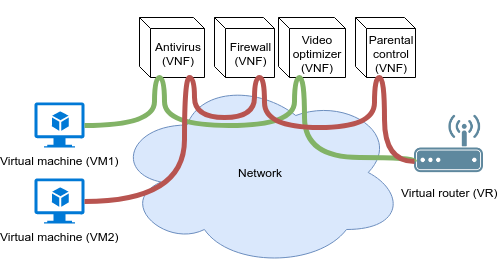
\includegraphics[width=0.95\textwidth]{vnf_chaining_example}
	\caption{--- Пример виртуального сетевого сервиса}
	\label{pic:vns_example}
\end{figure}

% Аналогию можно провести с математическим понятием функции. Пусть $x$ -- это входящие в сетевой сервис $S$ пакеты трафика. Тогда результатом работы сервиса $S$, состоящего из цепочки функций $f_{1} \to f_{2} \to f_{3}$ будет исходящий трафик $y$, такой что:
% \begin{equation}
% 	\label{eq:service_example}
% 	y = f_3(f_2(f_1(x))) = S(x)
% \end{equation}
% В результате пакеты $x$ трансформировались в пакеты $y$, где $S$ -- это суперпозиция функций $f_{1}$, $f_{2}$, $f_{3}$. 

% Таким образом, виртуальный сетевой сервис состоит из цепочки виртуальных сетевых функций, где работу каждой $i$-ой VNF можно представить в виде некоторого распределенного приложения $a_{i}$, которое обрабатывает сетевой трафик с помощью функции $f_{i}$. Цепочка таких приложений также образует некоторое абстрактное приложение $A$, которое обрабатывает трафик с помощью функции $S$. 

% В ходе неправильного использования приложения $A$ или же из-за ошибок, допущенных разработчиками, может случиться, что результаты работы приложения не совпадают с ожидаемыми результатами. При детектировании таких несоответствий мы будем искать причину с помощью  алгоритма, описанного в следующем разделе.





\chapter{Постановка задачи}
\section{Цель работы}
Целью данной работы является разработка системы валидации виртуальных сетевых сервисов для NFV платформы. 
\section{Задачи}
Для достижения поставленной цели следует решить следующие задачи:
% \begin{itemize}
%     \item провести обзор существующих решений;
%     \item разработать алгоритм валидации виртуальных сетевых сервисов;
%     \item разработать формат для хранения данных для проведения валидации;
%     \item разработать модуль проведения валидации виртуальных сетевых сервисов;
%     \item провести экспериментальное исследование.
% \end{itemize}
\begin{itemize}
    \item провести обзор существующих решений, выполняющих валидацию виртуальных сетевых сервисов;
    \item разработать и реализовать алгоритм валидации виртуальных сетевых сервисов;
    \item провести экспериментальное исследование эффективности разработанного алгоритма.
\end{itemize}






\chapter{Обзор существующих решений}
\label{chap:review-existed-solutions}
Перед тем, как приступить к разработке собственного решения, необходимо провести обзор существующих решений. Поэтому в данном разделе представлено краткое описание программных продуктов, решающих схожую задачу. Цель обзора --- выявить возможности существующих решений по валидации программного  обеспечения, виртуальных сетевых функций и виртуальных сетевых сервисов.

Здесь и далее по тексту будет использоваться понятие <<пользовательского требования>> как утверждение относительно характеристик субъекта. В данной работе субъектом является программное обеспечение, виртуальная сетевая функция или виртуальный сетевой сервис. Например, типичным требованием относительно виртуального сетевого сервиса может являться следующее: <<пропускная способность виртуального сетевого сервиса составляет 50 Мбит/c>>.

Также будет использоваться понятие <<валидация виртуальных сетевых функций>> как проверка пользовательских требований применительно к программному обеспечению, работающему на инфраструктуре, запущенной в NFV платформе как виртуальная сетевая функция. Понятие <<валидация виртуальных сетевых сервисов>> как проверка пользовательских требований применительно к совокупности виртуальных сетевых функций, входящих в состав сервиса.

Основное отличие валидации программного обеспечения от валидации виртуальных сетевых функций заключается в том, что для ПО в общем смысле отсутствуют ограничения и особенности, связанные с проведением проверки пользовательских требований. В то время как виртуальные сетевые функции представляют собой спецификацию управления жизненным циклом всего программно-аппаратного комплекса. Спецификация представлена на некотором языке и хранится в дескрипторе функции.

Ниже представлен обзор существующих решений.

\section{Open Platform for NFV}
Open Platform for NFV\cite{bib:opnfv} (OPNFV)  --- это платформа с открытым исходным кодом, на базе которой можно создавать компоненты  идеологии NFV. Проект OPNFV фокусируется на разработке менеджера инфраструктуры (NFVI) архитектуры ETSI NFV MANO. Основные цели проекта:
\begin{itemize}
	\item разработка интегрированной и протестированной открытой платформы, которая может быть использована для построения NFV, ускорения внедрения новых продуктов и сервисов;
	\item привлечение заинтересованных лиц со стороны конечных заказчиков для удовлетворения требований пользовательского сообщества;
	\item создание экосистемы NFV решений, основанной на открытых стандартах и программном обеспечении, которое удовлетворяет требованиям конечных пользователей;
	\item продвигать OPNFV как предпочтительную платформу и сообщество для создания NFV решений с открытым кодом.
\end{itemize}

OPNFV стремится участвовать в смежных открытых проектах, которые могут быть использованы в OPNFV для обеспечения целостности, высокой производительности и функциональной совместимости компонентов. OPNFV активно взаимодействует с открытыми проектами: OpenStack, KVM, Open vSwitch, OpenDaylight, ONOS, Open Contrail, ETSI, IETF. Сообщество состоит из более чем 60 компаний, начиная с производителей оборудования и заканчивая поставщиками SDN и NFV решений.

Первый релиз (Arno) состоялся в июне 2015 года и какой-либо функциональности в себе не нес.
Вторая версия проекта OPNFV (Brahmaputra) вышла 1 марта 2016 года. По словам сообщества, в платформе были реализованы поддержка тестирования производительности и другие средства проверки соответствия между требованиями приложений виртуальных сетевых функций и возможностями инфраструктуры. Таким образом, платформа готова для проведения лабораторных тестов. 

В рамках проекта OPNFV разрабатывается модуль VSperf, который представляет из себя инструмент для описания и проведения тестов над инфраструктурой. Инструмент включает в себя генераторы и анализаторы трафика, описание тестовых сценариев.

Как уже было отмечено, OPNFV -- это база для реализации продуктов на базе ETSI NFV MANO. В данной платформе разрабатывается лишь модуль NFVI, отвечающий за виртуальные ресурсы. Поэтому понятия виртуальная сетевая функция и виртуальный сетевой сервис здесь отсутствуют, а значит и отсутствует возможность их валидации.


\section{Cloudify}
Cloudify\cite{bib:cloudify} -- это платформа с открытым исходным кодом. Платформа архитектурно состоит из основного модуля, называемого Cloudify Manager VM, и Cloudify агентов, установленных на подконтрольных виртуальных машинах. 

Cloudify Manager VM ответственен за управление жизненным циклом виртуальных сетевых функций, а также выполняет роль оркестратора виртуальных сетевых функций. Таким образом, указанный модуль выполняет множество задач:
\begin{itemize}
	\item Регистрация новых виртуальных функций. Описание функций представляется в формате собственной разработки, называемый blueprints\cite{}. Он основан на стандарте описания функций TOSCA\cite{bib:tosca}.
	\item Размещение инфраструктуры VNF, используя плагины к существующим платформам виртуализации ресурсов (поддерживаются Openstack, VMware).
	\item Инициализация инфраструктуры функций. Используются программы-агенты на подконтрольных виртуальных машинах.
	\item Мониторинг изменения состояния виртуальных сетевых функций с помощью агентов.
	\item Запуск обработчика события из описания функции.
\end{itemize}

Cloudify агенты ответственны за выполнения команд от Cloudify Manager VM. Различают агентов со стороны Cloudify менеджера (manager side agents) и со стороны виртуальной сетевой функции (application side agents). Агенты менеджера устанавливаются вместе с операционной системой виртуальной машины и выполняют следующие служебные задачи: создание виртуальной машины, привязка внешнего ip-адреса и т.д.. Агенты виртуальной функции являются опцией (устанавливаются, если стоит соответствующая запись в описании функции). Задачи, выполняемые агентами функции, должны присутствовать в описании функции.

Анализ платформы показал, что в Cloudify не поддерживается проверка выполнения пользовательских требований к виртуальным сетевым функциям.


\section{OpenStack Tacker}
Openstack Tacker\cite{bib:openstack-tacker} -- это проект с открытым исходным кодом. Является дополнительным модулем для платформы виртуализации Openstack. Использует разработки проекта OPNFV. Основной целью проекта является реализация основных блоков ETSI NFV MANO\cite{bib:etsi-nfv-mano} (VNF-Manager и VNF-Orchestrator) в виде плагина для платформы виртуализации Openstack. Openstack Tacker реализует управление виртуальными сетевыми функциями и оркестрацию виртуальных сетевых сервисов.
	Рассмотрим основную функциональность базовых блоков архитектуры ETSI NFV MANO в рамках проекта Openstack Tacker. Основные задачи, выполняемые блоком VNF-Manager:
\begin{itemize}
	\item хранилище всех виртуальных функций, доступных системе;
	\item управление полным жизненным циклом каждой виртуальной функции (размещение, инициализация, масштабирование, остановка, удаление);
	\item мониторинг за размещенными виртуальными функциями (основные параметры мониторинга: производительность и отказоустойчивость функции);
	\item автоматическое восстановление работы функции в случае ее полного или частичного отказа в предоставлении услуги по заданным политикам;
	\item облегчение первоначальной настройки виртуальной сетевой функции.
\end{itemize}

Задачи, выполняемые блоком VNF-Orchestrator:
\begin{itemize}
	\item использование шаблонов при управлении сетевыми сервисами, комбинирование различных виртуальных сетевых функций между собой;
	\item обеспечение эффективного размещения виртуальных функций;
	\item создание цепочек виртуальных сетевых функций (сетевые сервисы);
	\item контроль за выделением ресурсов с помощью блока VIM;
	\item оркестрация виртуальных сетевых функций на множестве различных блоков VIM.
\end{itemize}

На текущий момент возможности Tacker реализованы только в режиме командной строки и не доступны в графическом интерфейсе Horizon платформы Openstack.

Восстановление работы функции и расширение инфраструктуры функции доступно только в ручном режиме. Интеграция с платформой виртуализации Openstack не позволяет использовать другие средства виртуализации инфраструктуры. Информации по валидации виртуальных сетевых функций или тем более виртуальных сетевых сервисов найдено не было.


\section{OpenBaton}
OpenBaton\cite{bib:openbaton} -- это проект с открытым исходным кодом, реализующий архитектуру ETSI NFV MANO. Основными модулями платформы являются:
\begin{itemize}
	\item оркестратор виртуальных сетевых сервисов NFVO;
	\item менеджер виртуальных сетевых функций VNFM;
\end{itemize}

Основным модулем, над которым ведется разработка --- NFVO. В нем содержится основная функциональность: размещение функций, слежение за их состоянием, восстановление из аварийного состояния и масштабирование. VNFM является заменяемым модулем: возможно использование модуля управления функциями собственной разработки. При этом с OpenBaton поставляются библиотеки, позволяющие упростить разработку и интегрирование собственного VNFM с оркестратором NFVO.

OpenBaton независима от платформы виртуализации ресурсов. На текущий момент разработан только плагин под платформу Openstack. Разработчиками заявлена поддержка одновременной работы с несколькими VIM. В OpenBaton для включения функции мониторинга необходимо дополнительно установить Zabbix сервер (о поддержке других решений по слежению за виртуальными машинами автору не известно).

% На момент написания работы в OpenBaton идет разработка следующей функциональности: развертывания дополнительной инфраструктуры и разнообразные улучшения в blueprints. Из этого следует, что о реализации автоматического масштабирования и восстановления функции речи пока не идет.

Для реализации собственных виртуальных сетевых сервисов OpenBaton предлагает либо реализовать менеджер функций собственной разработки, либо привести описании функции через VNFPackage. VNFPackage -- это дескриптор функции на основе формата YAML, который содержит необходимое описание виртуальной сетевой функции.

В документации к платформе также не было найдено какой-либо информации по валидации виртуальных сетевых функций и тем более виртуальных сетевых сервисов.


\section{Gym}
Gym\cite{bib:gym} -- это набор инструментов для тестирования производительности виртуальных сетевых функций. Разработка обладает следующими свойствами:
\begin{itemize}
    \item модульная архитектура с независимыми компонентами;
    \item простая система обмена сообщений с поддержкой удаленного вызова процедур (RPC);
    \item расширяемый набор инструментов тестирования и целевых метрик;
    \item определение тестов с помощью динамической композиции модулей;
    \item гибкие методы для вывода данных о тестировании и визуализации результатов.
\end{itemize}

Gym состоит из следующих модулей:
\begin{itemize}
    \item $Agent$. Обеспечивает расширенный интерфейс для инструментов тестирования (например, iperf\cite{}, ping\cite{}), позволяющих генерировать нагрузку на тестовый стенд.
    \item $Monitor$. Выполняет задачи по сбору статистики с помощью различных инструментов  (например, tcpdump\cite{}, top\cite{}).
    \item $Manager$. Отвечает за сохранения консистентности состояния всего модуля и обеспечивает координацию взаимодействия модулей $Agents$ и $Monitors$. Взаимодействует с модулем $Player$ для получения результатов тестирования, обработки результатов и формирования отчетов.
    \item $Player$. Представляет собой совокупность пользовательских интерфейсов для обработки запросов на тестирование и выдачи отчетов о тестировании обратно пользователю.
\end{itemize}

Основной вариант использования --- запуск тестирования производительности с последующим получением отчета с графиками производительности. Графиков производительности достаточно для проведения валидации пропускной способности виртуальных сетевых функций. Однако саму программу Gym для проведения исследования получить не удалось.


\section{Проприетарные решения}
Автору не известны проприетарные решения, реализующие валидацию виртуальных сетевых функций и/или виртуальных сетевых сервисов в рамках концепции NFV.


\section{Выводы}
Результаты обзора показали, что ни одно из обозреваемых решений не обладает механизмом валидации виртуальных сетевых сервисов. В таблице \ref{tab:nfv_platform_comprassion} приведены результаты обзора.

\renewcommand{\arraystretch}{1.5}
\begin{table}[h]
\center % центрирование таблицы
\begin{tabular}{|p{0.17\textwidth}|p{0.2\textwidth}|p{0.22\textwidth}|p{0.22\textwidth}|} % разделить колонки вертикальными линиями и центрировать содержимое каждой колонки
\hline % прочертить горизонтальную линию
Плат\-фор\-ма & Валидация ПО & Валидация VNF & Валидация VNS \\
\hline
OPNFV & + & - & - \\
\hline
Cloudify & - & - & - \\
\hline
Openstack Tacker & - & - & - \\
\hline
OpenBaton & - & - & - \\
\hline
Gym & - & +/- & - \\
\hline
\end{tabular}
\caption{--- Сравнение существующих решений.}
\label{tab:nfv_platform_comprassion}
\end{table}

% Однако на основании обзора можно сделать следующие выводы:
% \begin{itemize}
%     \item во всех проанализированных решениях виртуальные сетевые функции полностью определялись своим дескриптором;
%     \item некоторые решения предполагающие использование виртуальных сетевых сервисов (такие как OpenBaton) представляют использование 
% \end{itemize}

Таким образом, необходимо разработать собственное решение. В следующем разделе будет проведен анализ решения проблемы валидации виртуальных сетевых сервисов.





\chapter{Валидация виртуальных сетевых сервисов}
\label{chap:vns-validation}
Термин валидация означает процесс приведения доказательств того, что требования конкретного пользователя, продукта, услуги или системы удовлетворены. Строгое в математическом смысле доказательство в некоторых случаях оказывается достаточно сложным, а порой и невозможным. Например, достаточно сложно доказать, что пропускная способность между двумя точками в сети в любой момент времени будет не ниже заданной константы. А в случае если между конечными точками стоит устройство с неизвестным закрытым программным обеспечением, то верифицировать пропускную способность становиться невыполнимой задачей. В таких случаях проводят исследование интересующих сценариев использования. На основании такого исследования с учетом погрешностей принимается решение, выполняются пользовательские требования для конкретного сценария или нет.

Такая ситуация характерна и для виртуальных сетевых функций. В общем случае VNF --- это черный ящик, который потенциально может иметь бесконечное множество состояний. Поэтому невозможно в общем случае провести строгую проверку требований для любой виртуальной сетевой функции. Остается вариант с проведением исследования свойств VNF. Такое исследование включает в себя:
\begin{itemize}
    \item создание необходимого окружения для VNF;
    \item обеспечение достаточной нагрузки на VNF;
    \item обеспечение проверки выполнения требований.
\end{itemize}

Для автоматизированного проведения исследования свойств VNF необходимо разработать алгоритм и формат хранения данных для запуска алгоритма.

Напомним, что виртуальная сетевая функция представляется в платформе дескриптором, в котором хранится вся необходимая информация для управления ее жизненным циклом. Валидация также входит в понятие жизненный цикл виртуальной сетевой функции, поэтому данные для алгоритма проведения исследования будут храниться в дескрипторе функции. Напомним также, что дескриптор описывается на некотором языке, поэтому далее проведем обзор существующих языков спецификации виртуальных сетевых функций.



% хранить дополнительную информацию в дескрипторе функции:


% Для строгого доказательства, что конкретное требование выполняется для конкретного дескриптора виртуальной сетевой функции, необходимо построить модель

% проверить требование на всех возможных сценариях использования и на всех доступных виртуальной сетевой функции:
% \begin{itemize}
%     \item проверить требование на всех возможных сценариях использования виртуальной сетевой функции;
%     \item проверить требования 
% \end{itemize}

% Под требованием для программного обеспечения мы будем понимать успешное выполнение конкретного сценария использования с заданными ограничениями. Ограничениями могут быть следующими:
% \begin{itemize}
%     \item ограничение на интервал времени выполнения сценария;
%     \item ограничение на число затрачиваемых ресурсов;
%     \item ограничение на пропускную способность;
%     \item ограничение на сетевую задержку;
% \end{itemize}

% Указанное множества ограничений не является полным, однако часто используется на практике.

% Для проведения валидации необходимо

% В концепции NFV пользователь имеет дело с виртуальными сетевыми сервисами (VNS). Имеет смысл расширить свойства VNS, добавив в него поддержку пользовательских требований.

% Так как VNS структурно состоит из цепочек виртуальных сетевых функций, то соответствующие требования накладываются на VNFC. VNFC, в свою очередь, состоят из VNF. Таким образом, пользовательские требования должны выполняться для совокупности VNF, входящих в состав VNS. VNF является минимальным блоком в концепции NFV, поэтому проведем анализ возможности автоматической валидации пользовательских требования для VNF. Вся необходимая информация для автоматического управления жизненным циклом виртуальной сетевой функции содержится в VNF дескрипторе. Поэтому для реализации автоматической валидации пользовательских требований необходимо:
% \begin{itemize}
%     \item наличие дополнительной информации в дескрипторе функции;
%     \item поддержка валидации виртуальных сетевых функций в NFV платформе.
% \end{itemize}


\section{Обзор языков спецификации виртуальных сетевых функций}
\label{sec:review-vnf-languages}
Целью обзора является выявление возможности описания параметров для валидации виртуальных сетевых функций. Критерии обзора: 
\begin{itemize}
    \item встроенная поддержка хранения параметров валидации;
    \item возможность расширить формат для реализации поддержки хранения параметров валидации.
\end{itemize}

Далее будет приведено краткое описание каждого из рассматриваемых языков. 

\subsection{TOSCA}
TOSCA\cite{bib:tosca} представляет собой особую модель данных, которая описывается на одноименном языке. Дескриптор представляет собой файл в формате YAML\cite{bib:yaml}. В файле описываются операции автоматической установки, конфигурации, удаления и другие возможности управления приложением. В TOSCA все компоненты VNF представляются с помощью различных типов встроенных в язык отношений. Если встроенных типов недостаточно, то можно объявлять собственные.

В языке TOSCA отсутствуют встроенные типы для хранения информации о тестировании и валидации. Однако есть возможность реализовать собственный тип для хранения такой информации.

\subsection{JuJu}
Juju\cite{bib:juju:state} -- это инструмент для моделирования приложений, разработанный кампанией Canonical. Приложение позволяет уменьшить накладные расходы, связанные с размещением, настройкой, интеграцией и выполнением других рутинных задач в публичных и частных облачных сервисах. Juju также включает в себя одноименный язык для описания приложений, который позволяет абстрагироваться от трудоемкой настройки программного обеспечения. Все это позволяет уменьшить стоимость операций и обеспечивает гибкость. Пакет, в котором хранится описания приложения называется Charm. Он представляет собой файл конфигурации и сценариев настройки.

Juju позволяет указывать тестовые сценарии. По возвращаемому значению из сценария определяются, пройден тест (код 0), провален (код 1) или пропущен (код 100). Сценарий может быть написан на bash\cite{} или Python\cite{}. Других встроенных полей для хранения информации о тестировании не предусмотрено.

\subsection{YANG}
YANG\cite{bib:rfc:yang} -- это язык моделирования данных, который определяет как и что надо передать через сетевой протокол управления конфигурацией NETCONF\cite{bib:rfc:netconf}. Язык разработан рабочей группой NETMOD из Internet Engineering Task Force (IETF). YANG используется для моделирования данных конфигурации и состояния сетевых элементов. Более того, язык может использоваться для определения формата уведомлений о каких-либо событиях, происходящих в сетевых элементах, что позволяет использовать концепцию Remote Procedure Call (RPC).

Также язык может быть использован как язык спецификации виртуальных сетевых функций. В нем также не предусмотрено встроенных полей для хранении информации о тестировании.


\subsection{Cloudify Blueprint}
NFV платформа Cloudify использует собственный язык спецификации виртуальных сетевых функций, называемый Cloudify Blueprint\cite{bib:blueprint}. Blueprint представляет собой язык TOSCA с дополнительными типами для описания узлов, политик и различных параметров.
В остальном синтаксис и семантика соответствует TOSCA, дополнительных полей для хранения параметров валидации обнаружено не было.

\subsection{Heat Orchestration Template}
Heat Orchestration Template\cite{bib:hot} (HOT) представляет собой формат для хранения топологий с описанием параметров и ограничений размещения. В отличие от остальных языков HOT не позиционируется как язык спецификаций виртуальных сетевых функций, однако в нем есть возможность описать собственные ограничения, которые могут интерпретироваться как схемы настройки функции или же как политики управления, масштабирования, восстановления.

Как и в представленных выше языках здесь также отсутствуют встроенные механизмы для хранения параметров валидации.


\subsection{Выводы}
На данным момент почти каждая NFV платформа разрабатывает собственный язык спецификации виртуальных сетевых функций. Однако все рассмотренные языки имеют схожий формат и одну общую идею спецификации параметров. 

Результаты обзора показали, что в рассмотренных языках отсутствует встроенная поддержка валидации виртуальных сетевых функций. Однако каждый из языков обладает достаточной мощностью для описания дополнительных сценариев и других параметров для проведения валидации виртуальных сетевых функций. Ниже представлена таблица \ref{tab:language-overview} с результатами обзора.

\renewcommand{\arraystretch}{1.5}
\begin{table}[h]
\center % центрирование таблицы
\begin{tabular}{|p{0.25\textwidth}|p{0.3\textwidth}|p{0.33\textwidth}|} % разделить колонки вертикальными линиями и центрировать содержимое каждой колонки
\hline % прочертить горизонтальную линию
Язык & Встроенная поддержка валидации & Возможность добавления параметров валидации \\
\hline
TOSCA & - & + \\
\hline
Juju & - & + \\
\hline
YANG & - & + \\
\hline
Cloudify Blueprint & - & + \\
\hline
HOT & - & + \\
\hline
\end{tabular}
\caption{--- Сравнение языков спецификации}
\label{tab:language-overview}
\end{table}

Таким образом, выбор языка спецификации не влияет на возможность реализации системы валидации. В любом из форматов можно организовать хранение данных, необходимых для проведения валидации виртуальных сетевых сервисов. Далее будет описана схема валидации виртуальных сетевых функций.


\section{Алгоритм валидации виртуальных сетевых функций}
\label{sec:vnf-validation-algotihm}
В рамках данной работы был разработан алгоритм валидации пропускной способности виртуальных сетевых функций. Детальная схема алгоритма представлена на рисунке \ref{pic:analyse_vnf_algorithm}.

\begin{figure}[h]
	\centering
	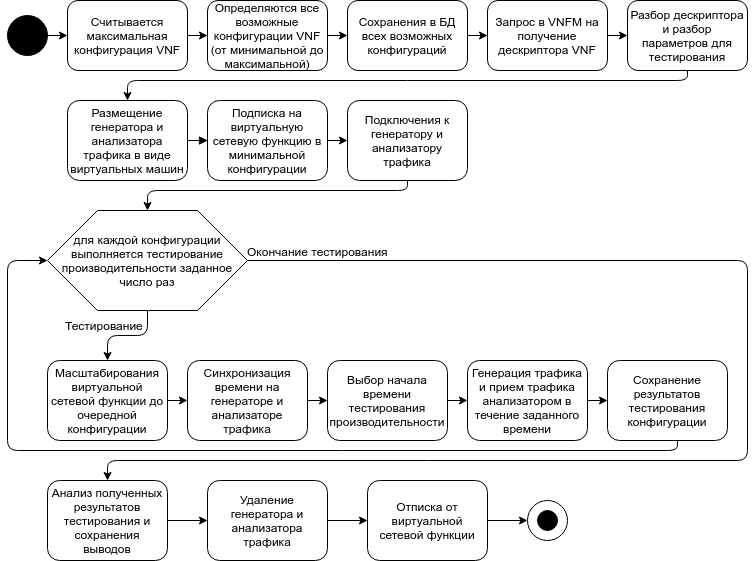
\includegraphics[width=0.95\textwidth]{analyse_vnf_algorithm}
	\caption{--- Алгоритм валидации виртуальной сетевой функции}
	\label{pic:analyse_vnf_algorithm}
\end{figure}

Алгоритм работает в следующих предположениях:
\begin{itemize}
    \item Виртуальная сетевая функция масштабируется поэтапно, начиная с минимальной конфигурации и заканчивая максимальной (определяется параметром при запросе на анализ).
    \item Виртуальная сетевая функция масштабируется строго по возрастанию производительности. 
    \item Все множество доступных ресурсов делится на три типа: ядра процессора, размер оперативной и постоянной памяти. Предполагается, что используются одинаковые процессоры, оперативная и постоянная память с одинаковыми характеристиками.
    \item Максимальная конфигурация исследуемой функции задается в запросе (входной параметр).
    \item Времени тестирования одной конфигурации задается в запросе (входной параметр).
    \item Количество итераций тестирования задается в запросе (входной параметр).
    \item Виртуальная сетевая функция должна быть зарегистрирована в NFV платформе.
    \item Производительности генератора и анализатора трафика достаточно для поддержки любого пользовательского требования. В случае, если одна виртуальная машина генератора и/или анализатора трафика не справляется, то можно поднять несколько экземпляров виртуальных машин генераторов и/или анализаторов трафика.
\end{itemize}


\section{Алгоритм валидации виртуальных сетевых сервисов}
Как было сказано в разделе \ref{sec:vns} виртуальный сетевой сервис -- это совокупность функций, которые связанны между собой в цепочки. В начале цепочки ставится классификатор, который определяет, какой трафик пойдет в цепочку. 

Под пользовательским требованием к виртуальному сетевому сервису мы будем понимать требование к каждой цепочке внутри этого сервиса. В свою очередь требование к цепочке -- это требование к каждой отдельно взятой виртуальной сетевой функции, входящей в состав цепочки. Таким образом, требование к сервису -- это требование к каждой функции, входящей в состав рассматриваемого сервиса.

Алгоритм валидация виртуального сетевого сервиса состоит из следующих шагов:
\begin{itemize}
    \item ввести пользовательское требование, ограничение по числу используемых ресурсов (количество ядер, размер оперативной и постоянной памяти) и структуру виртуального сетевого сервиса (все цепочки функций); 
    \item проанализировать, из каких виртуальных сетевых функций состоит сервис;
    \item проверить, что для каждой функции существует конфигурация, в которой выполняется пользовательское требование, и выбрать минимальную такую конфигурацию, в противном случае сообщить о невозможности предоставить валидный виртуальный сетевой сервис;
    \item просуммировать все выбранные конфигурации функций и проверить, что выполняется ограничение по затрачиваемым ресурсам;
    \item в случае успеха вернуть все выбранные конфигурации функций, в противном случае сообщить о невозможности предоставить валидный виртуальный сетевой сервис.
\end{itemize}

Таким образом, данный алгоритм позволяет решить задачу валидации пропускной способности для виртуальных сетевых сервисов. В следующих двух разделах представлены требования к разрабатываемому решению и описание реализации алгоритма для NFV платформы С2 Platform\cite{bib:c2-platform}.





\chapter{Требование к решению}
На основании обзоров из разделов \ref{chap:review-existed-solutions} и \ref{sec:review-vnf-languages} и алгоритма, приведенного в \ref{sec:vnf-validation-algotihm}, разрабатываемое решение должно:
\begin{itemize}
    \item выдавать конфигурацию виртуальной сетевой функции, удовлетворяющую заданным пользовательским требованиям;
    \item выдавать конфигурацию виртуального сетевого сервиса, удовлетворяющего заданным пользовательским требованиям;
    \item проводить анализ свойств виртуальных сетевых функций.
\end{itemize}





\chapter{Описание практической части}
\label{chap:practice}
В текущей главе приведено описание реализации алгоритма валидации виртуальных сетевых сервисов для NFV платформы С2 Platform\cite{bib:c2-platform}. Проект разрабатывается отечественной организацией Центр Прикладных Исследований Компьютерных Сетей (ЦПИКС)\cite{bib:arccn}.


\section{Облачная платформа C2 Platform}
\label{sec:c2-platform-description}
Рассматриваемая NFV платформа реализована по высокоуровневой архитектуре ETSI NFV MANO. Взаимодействие между внутренними модулями осуществляется через библиотеку RabbitMQ\cite{bib:rabbitmq} (RMQ). 

Проект C2 Platform состоит из нескольких модулей следуя парадигме миркосервисов:
\begin{itemize}
	\item веб-интерфейс платформы (GUI-сlient);
	\item модуль, предоставляющий интерфейс для OSS/BSS систем (GUI-server);
	\item модуль виртуализации инфраструктуры (VIM);
	\item модуль мониторинга (Mon);
	\item менеджер функций (VNFM);
	\item оркестратор сервисов (Orch);
\end{itemize}

Далее представлено подробное описание модулей платформы C2.

\subsection{Графический интерфейс}
Оба модуля (GUI-client и GUI-server) отвечают за:
\begin{itemize}
	\item отображение актуальной информации о текущей загрузке физических серверов;
	\item отображение размещенных тенантов (тенант -- это сети виртуальных машин);
	\item авторизацию пользователей;
	\item предоставление управления виртуальными сетевыми функциями и виртуальными сетевыми сервисами;
	\item отображение актуального состояния виртуальных сетевых функций и сервисов.
\end{itemize}

Модуль GUI-server является поставщиком данных для GUI-client. В нем сосредоточены все основные интерфейсы C2 Platform. 

\subsection{Модуль виртуализации ресурсов}
Модуль VIM состоит из двух основных частей: плагин для существующей платформы виртуализации ресурсов (используется Openstack) и независимая часть для обработки сообщений от других модулей проекта C2 Platform (Mon, VNFM, GUI-server и т.д.). Плагин можно менять в зависимости от используемой платформы виртуализации ресурсов (Openstack, VMWare и т.д.). Задача второй части заключается в управлении тенантами (сеть с виртуальными машинами) по запросу от других модулей платформы. 

Основные интерфейсы для других модулей: 
\begin{itemize}
    \item размещение и удаление тенанта;
    \item предоставление консоли к конкретной виртуальной машине;
    \item предоставление различной информации о:
    \begin{itemize}
        \item размещенных сетях и виртуальных машинах;
        \item занятых ресурсах;
        \item реализации цепочек виртуальных сетевых функций.
    \end{itemize}
\end{itemize}

\subsection{Модуль мониторинга}
Модуль мониторинга Mon так же состоит из двух частей: плагин для существующей программы мониторинга (используется Zabbix \cite{bib:zabbix}) и независимая часть для обработки сообщений от других модулей проекта C2 Platform (GUI-server, VNFM, и т.д.). Плагин можно менять в зависимости от используемой программы мониторинга. Независимая часть обеспечивает слежение за виртуальными машинами и соединениями между ними.

Основные интерфейсы для других модулей: установка и удаление мониторов за виртуальными машинами, оповещение подписанных модулей о событиях, предоставление статистики по работе виртуальных машин.

\subsection{Модуль оркестрации сервисов}
Модуль оркестрации виртуальных сетевых сервисов Orch занимается управлением цепочек сетевых функций, отправляя запросы к модулям VIM и VNFM. Имея возможность взаимодействовать сразу с несколькими модулями VIM, оркестратор, исходя из текущей загруженности доступных ЦОД, решает, куда необходимо разместить очередную цепочку. В текущей реализации имеется возможность размещать одну цепочку сетевых функций на инфраструктуре одного виртуального ЦОД (инфраструктурой одного виртуального ЦОД управляет один модуль VIM).

Основной интерфейс, предоставляемый модулем: размещение, удаление, изменение виртуальных сетевых сервисов.

\subsection{Модуль управления виртуальными сетевыми функциями}
Модуль управления виртуальными сетевыми функциями VNFM состоит из двух основных частей: анализатор спецификаций виртуальных сетевых функций и часть для взаимодействия с другими модулями проекта C2 Platform (Orch, VNFM). Модуль умеет регистрировать виртуальные сетевые функции, внося соответствующую информацию в базу данных. Модуль анализирует дескриптор функции и занимается конфигурацией ее инфраструктуры.

Основной интерфейс, предоставляемый модулем: управление, конфигурирование и поддержка виртуальных сетевых функций.


\section{Реализация модуля валидации}
\label{sec:developed_module}
Модуль валидации виртуальных сетевых сервисов был реализован как отдельный модуль, так как не является обязательным модулем высокоуровневой архитектуры ETSI NFV MANO. 

В дополнении к остальным модулям NFV платформы, разработка позволяет проводить анализ виртуальных сетевых функций, запоминать его результаты и затем использовать их для валидации виртуальных сетевых сервисов. Диаграмма классов разработанного модуля представлена на рисунке \ref{pic:validation_classes_diagram} ниже.

\begin{figure}[h]
	\centering
	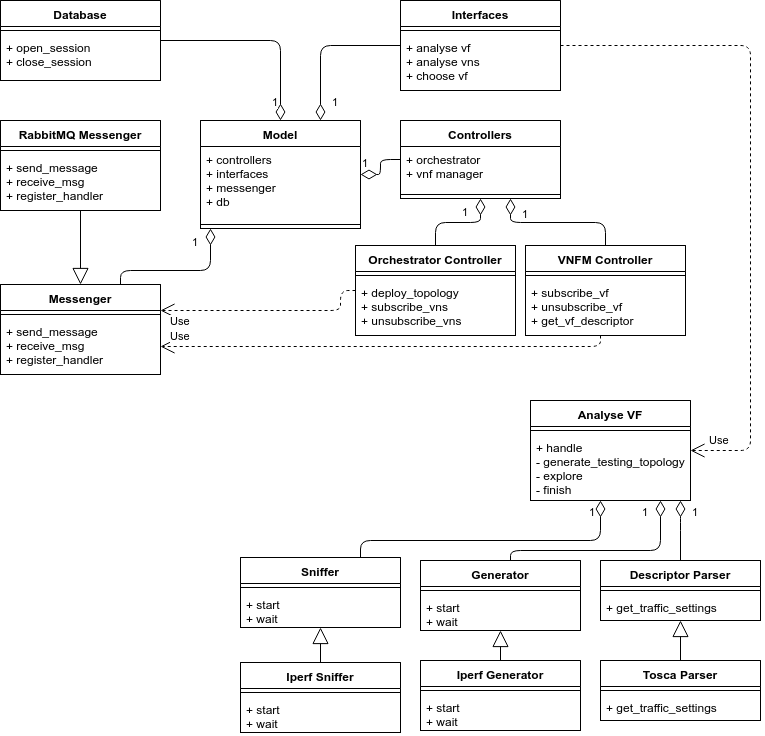
\includegraphics[width=0.95\textwidth]{classes_diagram}
	\caption{--- Диаграмма классов модуля валидации}
	\label{pic:validation_classes_diagram}
\end{figure}

Типичное использование модуля валидации выглядит следующим образом:
\begin{itemize}
    \item предварительная регистрация виртуальных сетевых функций, которые будут использоваться;
    \item запуск анализа виртуальных сетевых функций;
    \item запрос на подписку на виртуальной сетевой сервис с указанием требования по пропускной способности
    \item в случае успеха можно использовать валидный виртуальный сетевой сервис, в противном случае --- нельзя разместить валидный сервис.
\end{itemize}

В следующей главе приведено описание экспериментального исследования.





\chapter{Экспериментальное исследование}
\label{chap:expirements}
В рамках данной работы проводилось исследование влияния разработанного модуля валидации на время получения стабильной подписки на виртуальный сетевой сервис. 

Подпиской на виртуальный сетевой сервис мы будем называть запрос в NFV платформу на предоставление функциональности перечисленных в сервисе виртуальных сетевых функций. Стабильной подпиской мы будем называть такую подписку на виртуальный сетевой сервис, когда ни одна виртуальная сетевая функция не будет под текущей нагрузкой масштабироваться.


\section{Описание}
Проведем эксперименты с виртуальным сетевым сервисом, состоящим из одной виртуальной сетевой функции Snort\cite{bib:snort}. Для функции установлены политики масштабирования, которые добавляют дополнительную виртуальную машину с функцией Snort в случае, когда пропускная способность на интерфейсе превышает заданную величину (70 Мбит/с) в течение заданного времени (10 секунд). В качестве инфраструктуры будет использоваться виртуальная машина с сетевыми интерфейсами 100 Мбит/c.

Разместим генератор и приемник трафика в виде двух виртуальных машин с предустановленной утилитой iperf\cite{bib:iperf}. Сделаем подписку на виртуальный сетевой сервис, состоящий из одной цепочки от генератора до приемника из одной функции Snort. Установим пользовательское требование на уровень 400 Мбит/c.

В эксперименте без использования разработанного модуля валидации виртуальная сетевая функция Snort сначала была размещена в минимальной конфигурации. Затем NFV платформа 4 раза произвела масштабирование указанной функции. В результате итоговая конфигурация функции составила 5 виртуальных машин с одинаковой конфигурацией.

В эксперименте с использованием разработанного модуля валидации подписка осуществлялась с указанием требования по пропускной способности в 400 Мбит/c. В результате подписки виртуальная сетевая функция Snort сразу разместилась в конфигурации из пяти одинаковых виртуальных машин.


\section{Выводы}
Всего проводилось 10 экспериментов с использованием модуля валидации и 10 экспериментов без него. Результаты приведены в таблице \ref{tab:expirement-time} ниже. $T$ --- это время получения стабильного виртуального сетевого сервиса в эксперименте. $\Expect (T)$ --- среднее время по всем экспериментам. $Min(T)$ --- минимальное время по всем экспериментам. $Max(T)$ --- максимальное время по всем экспериментам.

\renewcommand{\arraystretch}{1.5}
\begin{table}[h]
\center % центрирование таблицы
\begin{tabular}
{|p{0.25\textwidth}|p{0.17\textwidth}|p{0.14\textwidth}|p{0.17\textwidth}|} % разделить колонки вертикальными линиями и центрировать содержимое каждой колонки
\hline % прочертить горизонтальную линию
% & $\Variance (T) $, сек
Использование модуля валидации & $Min(T)$, сек & $\Expect (T)$, сек & $Max(T)$, сек \\
\hline
используется & 54 & 55 & 56 \\
\hline
не используется & 213 & 224 & 239 \\
\hline
\end{tabular}
\caption{--- Время на получение стабильного сервиса.}
\label{tab:expirement-time}
\end{table}

Таким образом, использование модуля валидации позволило ускорить процесс получение стабильного виртуального сетевого сервиса в проведенных экспериментах примерно в 4 раза. Так как NFV платформа предварительно провела анализ виртуальных сетевых функций, входящих в состав сервиса, то сервис, полученный с использованием разработанного модуля, отвечает пользовательским требования в 400 Мбит/c.





\chapter*{Заключение}
\addcontentsline{toc}{chapter}{Заключение} % добавить Заключение в оглавление
В рамках данной работы был разработан алгоритм валидации виртуальных сетевых сервисов.

В разделе \ref{chap:nfv} было представлено краткое введение в концепцию NFV. Далее в разделе был проведен обзор существующих решений \ref{chap:review-existed-solutions}, в \ref{chap:vns-validation} проведен анализ, как и где можно хранить данные для проведения валидации, и представлен алгоритм для валидации виртуальных сетевых функций и сервисов. Затем в \ref{chap:practice} представлено описание практической части работы и, наконец, в \ref{chap:expirements} представлено описание экспериментального исследования.

Разработанное решение позволяет проводить валидацию виртуальных сетевых сервисов на пользовательских требованиях, связанных с пропускной способностью виртуальных сетевых сервисов.

Дальнейшие исследования в области валидации виртуальных сетевых сервисов можно продолжать по нескольким направлениям: 

\begin{itemize}
    \item расширение числа метрик, по которым можно задавать пользовательские требования;
    \item поддержка вертикальной и горизонтальной масштабируемости виртуальных сетевых функций;
    \item расширение числа средств, с помощью которых можно проводить генерацию и анализ трафика.
\end{itemize}




% Список литературы
\begin{thebibliography}{00}
\addcontentsline{toc}{chapter}{Литература}
\bibitem{bib:nfv:white-paper} Cui C. et al. Network Functions Virtualisation.
\bibitem{bib:etsi-nfv-mano} Ersue M. ETSI NFV management and orchestration-An overview //Proc. of 88th IETF meeting. – 2013.
% \bibitem{bib:google-app-engine} Google App Engine; Alexander Zahariev; Helsinki University of Technology;  April, 2009.
% \bibitem{bib:tosca} TOSCA Simple Profile in YAML Version 1.0; Standards Track Work Product; OASIS Open 2016; December 2016.
\bibitem{bib:rfc:yang} Bjorklund M. RFC 6020: YANG-a data modeling language for the network configuration protocol //IETF. – 2010.
% \bibitem{bib:rfc:validation} Walden D. D. et al. Systems engineering handbook: A guide for system life cycle processes and activities. – John Wiley \& Sons, 2015.
\bibitem{bib:tosca} TOSCA O. TOSCA Simple Profile for Network Functions Virtualization (NFV) Version 1.0. – 2015.
\bibitem{bib:juju:state} Wettinger J., Andrikopoulos V., Leymann F. Automated capturing and systematic usage of devops knowledge for cloud applications //Cloud Engineering (IC2E), 2015 IEEE International Conference on. – IEEE, 2015. – С. 60-65.
\bibitem{bib:blueprint} Fernandez Afonso C. E. An elasticity controller for applications orquestrated with Cloudify : дис. – 2016.
\bibitem{bib:hot} Yamato Y. et al. Development of template management technology for easy deployment of virtual resources on OpenStack //Journal of Cloud Computing. – 2014. – Т. 3. – №. 1. – С. 7.
\bibitem{bib:rfc:netconf} Enns R. RFC 4741: NETCONF Configuration Protocol, 2006.
\bibitem{bib:gym} Rosa R. V., Bertoldo C., Rothenberg C. E. Take Your VNF to the Gym: A Testing Framework for Automated NFV Performance Benchmarking //IEEE Communications Magazine. – 2017. – Т. 55. – №. 9. – С. 110-117.



% \bibitem{nfv-official} Network Functions Virtualization; white paper; ETSI; October, 2012.
% \bibitem{bib:openstack} OpenStack, OpenStack Compute Admin Manual Manual, November 2011.
% \bibitem{bib:vmware} Memory Resource Management in VMware ESX Server; C. Waldspurger; Operating Systems Design and Implementation (OSDI); 2002.
% \bibitem{nfv-state1} NFV виртуализация сетевых функций (дата обращения 1 мая 2017 года) [HTML] (http://sci-article.ru/stat.php?i=1455156066).
% \bibitem{opnfv-official} OPNFV - An open platform to accelerate NFV; Linux Foundation; October, 2014.
\bibitem{bib:cloudify} Chappell C. NFV MANO: What's Wrong \& How to Fix It //Heavy Reading. – 2015. – Т. 13. – №. 2.
\bibitem{bib:opentack-tacker} Hoang C. P. et al. Monitoring driver for container-based VNFs in OpenStack Tacker. – 2017. – С. 1459-1460.
% \bibitem{bib:tosca} TOSCA Simple Profile in YAML Version 1.0; Standards Track Work Product; OASIS Open 2016; December 2016.
\bibitem{bib:opnfv} Price C. et al. Opnfv: An open platform to accelerate nfv //White Paper. A Linux Foundation Collaborative Project. – 2012.
\bibitem{bib:snort} Coit C. J., Staniford S., McAlerney J. Towards faster string matching for intrusion detection or exceeding the speed of snort //DARPA Information Survivability Conference \& Exposition II, 2001. DISCEX'01. Proceedings. – IEEE, 2001. – Т. 1. – С. 367-373.
\bibitem{bib:arccn} TODO
\bibitem{bib:openbaton} Baton O. Open baton: an open source reference implementation of the etsi network function virtualization mano specification.
\bibitem{bib:yaml} Ben-Kiki O., Evans C., Ingerson B. Yaml ain't markup language (yaml™) version 1.1 //yaml. org, Tech. Rep. – 2005. – С. 23.
\bibitem{bib:c2-platform} Antonenko, V., Smeliansky, R., Ermilov, A., Plakunov, A., Pinaeva, N., Romanov, A.. C2: General Purpose Cloud Platform with NFV Life-Cycle Management //Cloud Computing Technology and Science (CloudCom), 2017 IEEE International Conference on. – IEEE, 2017. – С. 353-356.
\bibitem{bib:zabbix} Zabbix S. I. A. Zabbix. The Enterprise-class Monitoring Solution for Everyone. – 2014.
\bibitem{bib:iperf} Hsu C. H., Kremer U. IPERF: A framework for automatic construction of performance prediction models //Workshop on Profile and Feedback-Directed Compilation (PFDC), Paris, France. – 1998.
\bibitem{bib:rabbitmq} Videla A., Williams J. J. W. RabbitMQ in action: distributed messaging for everyone. – Manning, 2012.
\end{thebibliography}

% Конец документа
\end{document}